\documentclass[letter,12pt]{article}
\usepackage[letterpaper,right=1in,left=1in,top=1in,bottom=1in]{geometry}
\usepackage{setspace}

\usepackage[utf8]{inputenc}   % allows input of special characters from keyboard (input encoding)
\usepackage[T1]{fontenc}      % what fonts to use when printing characters       (output encoding)
\usepackage{amsmath}          % facilitates writing math formulas and improves the typographical quality of their output
\usepackage[hyphens]{url}     % adds line breaks to long urls
\usepackage[pdftex]{graphicx} % enhanced support for graphics
\usepackage{tikz}             % Easier syntax to draw pgf files (invokes pgf automatically)
\usetikzlibrary{arrows}

\usepackage{mathptmx}           % set font type to Times
\usepackage[scaled=.90]{helvet} % set font type to Times (Helvetica for some special characters)
\usepackage{courier}            % set font type to Times (Courier for other special characters)

\usepackage[longnamesfirst, sort]{natbib}\bibpunct[]{(}{)}{,}{a}{}{;} % handles biblio and references 

\usepackage{rotating}         % sideway tables and figures that take a full page
\usepackage{caption}          % allows multipage figures and tables with same caption (\ContinuedFloat)

\usepackage{dcolumn}          % needed for apsrtable and stargazer tables from R to compile
\usepackage{arydshln}         % dashed lines in tables (hdashline, cdashline{3-4}, 
                              %see http://tex.stackexchange.com/questions/20140/can-a-table-include-a-horizontal-dashed-line)
                              % must be loaded AFTER dcolumn, 
                              %see http://tex.stackexchange.com/questions/12672/which-tabular-packages-do-which-tasks-and-which-packages-conflict


\newcommand{\mc}{\multicolumn}

%% TO ADD NOTES IN TEXT, PUT % BEFORE THE ONE YOU WANT DISABLED
\usepackage[disable]{todonotes}                            % no show
%\usepackage[colorinlistoftodos, textsize=small]{todonotes} % show notes
\newcommand{\emm}[1]{\todo[color=red!15, inline]{\textbf{Eric:} #1}}
\newcommand{\vp}[1]{\todo[color=green!15, inline]{\textbf{Vale:} #1}}
\newcommand{\ges}[1]{\todo[color=blue!15, inline]{\textbf{Ges:} #1}}

\usepackage{xr} % allows cross-ref to other file
\externaldocument{urge15appendix}
\setcitestyle{citesep={;}}
\usepackage{listings}

\begin{document}

\section{Paste in paper}



DV


\singlespacing
\begin{footnotesize}
\begin{verbatim}
| Members in office                                       |   % |    N |
|---------------------------------------------------------+-----+------|
| one observed Legislatura only                           |  86 | 1470 |
| one observed and one or more unobserved Legislaturas    |   9 |  149 |
| two observed (and zero or more unobserved) Legislaturas |   5 |   91 |
| three observed Legislaturas                             |   0 |    0 |
|---------------------------------------------------------+-----+------|
| Total                                                   | 100 | 1710 |
\end{verbatim}
\end{footnotesize}
\doublespacing

The table offers contrast between diputados and presiding officers, adopting members as units instead of daily sessions, as above. Speechless members, who remain unobserved in session-level data, are now accounted for. Of 1,710 members observed across the three Legislaturas, 156 never uttered a single word in the plenary throughout their tenure. The median member spoke 3,677 words in total, the median presiding officer spoke 46,710. Since tenure lengths vary (91 members, or 5 percent of all, were present in two of the Legislaturas observed), a relative measure is desirable. The median diputado spoke 26.4 words per session on average, while the median presiding officer spoke an average 258.6 words per session. Presiding officers are therefore dropped from the analysis. 

95 percent of members never served as presiding officers. Of those who did, the mode was 

\singlespacing
\begin{footnotesize}
\begin{verbatim}
| Years as presiding officer |   % |    N |
|----------------------------+-----+------|
| never                      |  95 | 1630 |
| one                        |   3 |   49 |
| two                        |   1 |   19 |
| three                      |   1 |   12 |
|----------------------------+-----+------|
|                            | 100 | 1710 |
\end{verbatim}
\end{footnotesize}
\doublespacing


\singlespacing
\begin{footnotesize}
\begin{verbatim}
* * Member descriptives for diputados vs presiding officers * *
|                       |  min |   25% |   50% |   75% |    max |
|-----------------------+------+-------+-------+-------+--------|
| DIPUTADOS             |      |       |       |       |        |
| Total words in period |    0 |  1128 |  3677 |  8535 | 242434 |
| Sessions in office    |    1 |   121 |   180 |   201 |    522 |
| Words by session      |    0 |   9.9 |  26.4 |  57.4 | 1212.2 |
|-----------------------+------+-------+-------+-------+--------|
| PRESIDING OFFICERS    |      |       |       |       |        |
| Total words in period | 3141 | 25680 | 46710 | 71669 | 320155 |
| Sessions in office    |   32 |   121 |   182 |   219 |    522 |
| Words by session      | 19.6 | 137.7 | 258.6 | 436.5 | 3563.3 |

* * Member descriptives for diputados vs presiding officers * *
|                       |  min |   10% |   25% |   50% |   75% |    90% |    max |
|-----------------------+------+-------+-------+-------+-------+--------+--------|
| DIPUTADOS             |      |       |       |       |       |        |        |
| Total words in period |    0 |   135 |  1128 |  3677 |  8535 |  16948 | 242434 |
| Sessions in office    |    1 |    25 |   121 |   180 |   201 |    219 |    522 |
| Words by session      |    0 |   1.1 |   9.9 |  26.4 |  57.4 |  109.2 | 1212.2 |
|-----------------------+------+-------+-------+-------+-------+--------+--------|
| PRESIDING OFFICERS    |      |       |       |       |       |        |        |
| Total words in period | 3141 | 13046 | 25680 | 46710 | 71669 | 148511 | 320155 |
| Sessions in office    |   32 |   121 |   121 |   182 |   219 |    227 |    522 |
| Words by session      | 19.6 |  80.9 | 137.7 | 258.6 | 436.5 |  802.0 | 3563.3 |

\end{verbatim}
\end{footnotesize}
\doublespacing




\subsection{N speakers}

\begin{figure}
  \centering
    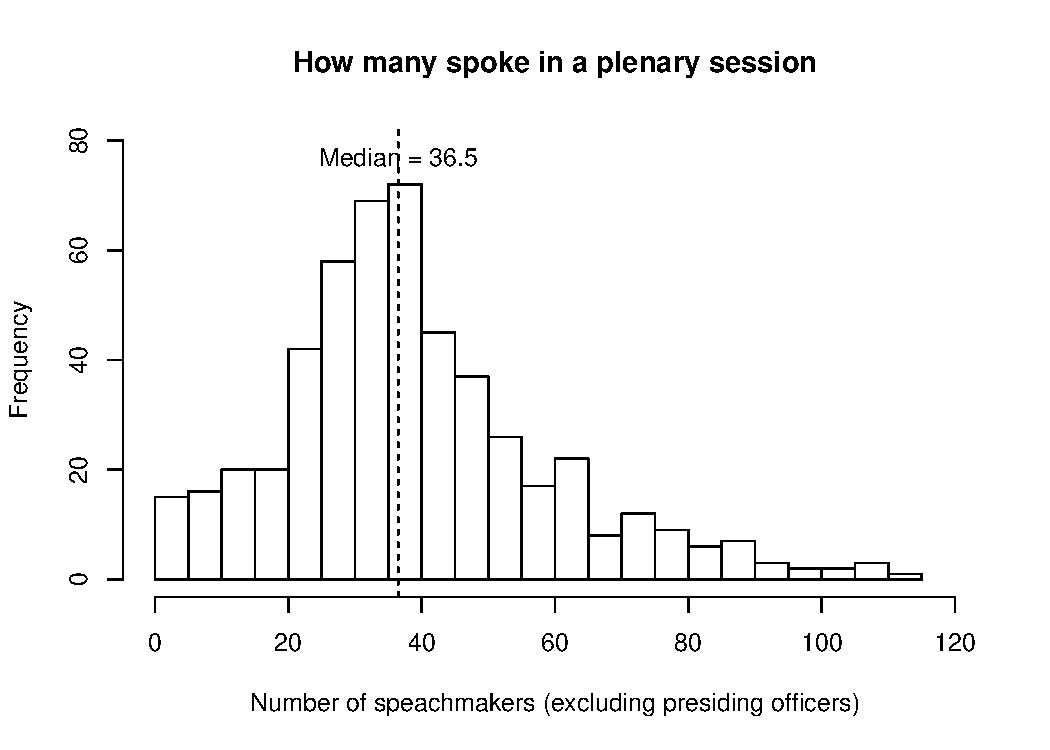
\includegraphics[width=.8\columnwidth]{../plots/nspeakers.pdf}
    \caption{How many spoke in the plenary? Daily plenary sessions of the 60th, the 62nd, and the first two years of the 64th Legislaturas.}\label{F:nspeakers}
\end{figure}





\listofendnotes

\bibliographystyle{apsr}

\bibliography{../bib/magar}

%% \begin{thebibliography}{xx}

%% \harvarditem{Alem\'an \harvardand\ Tsebelis}{2016}{aleman-tsebelis-2016-book}
%% Alem\'an, Eduardo \harvardand\ George Tsebelis. 2016.
%% \newblock {\em Legislative Institutions and Lawmaking in Latin America}.
%% \newblock Oxford:  Oxford University Press.

%% \harvarditem{Alem\'an \harvardand\ Navia}{2009}{aleman.navia.UrgChi.2009}
%% Alem\'an, Eduardo \harvardand\ Patricio Navia. 2009.
%% \newblock ``Institutions and the Legislative Success of `Strong' Presidents: An
%%   Analysis of Government Bills in {Chile}.'' {\em Journal of Legislative
%%   Studies} 15(4):401--19.

%% \end{thebibliography}


\end{document}

